\chapter{Druck der Teile}
Im Folgenden wird der eigentliche 3D-Druck der Bauteile näher erläutert. Hierzu wird zunächst näher auf das Verfahren eingegangen, anschließend werden verschiedene Einstellungsmöglichkeiten bei der Erstellung der Steuercodes für den 3D-Drucker gezeigt.

\section{Druck}

\subsection{FDM}
Der Druck der Teile wurde bei dem hier vorgestellten Projekt nach dem \ac{FDM}-Verfahren durchgeführt, welches bereits 1989 durch S. Scott Crump mit der Firma Stratasys, Inc. patentiert\footnote{\cite{Crump1992}} wurde. Erst durch die auslaufenden Patentrechte wurde eine freie Verfügbarkeit ermöglicht. Auf diesem Verfahren basieren heute die Meisten 3D-Drucker in Preisklassen bis hin zum oberen Mittelfeld.

Bei dem \ac{FDM}-Verfahren wird das Ausgangsmaterial verflüssigt und durch eine ca. 0.4mm große Öffnung im Druckkopf gepresst. Durch eine Bewegung in 3-Achsen wird das flüssige Material in ca. 0.05 - 0.35mm dicken Schichten auf eine Plattform aufgetragen, dabei verschmelzen die Schichten miteinander und bilden das fertige Modell.

\begin{figure}[h]
  \centering
  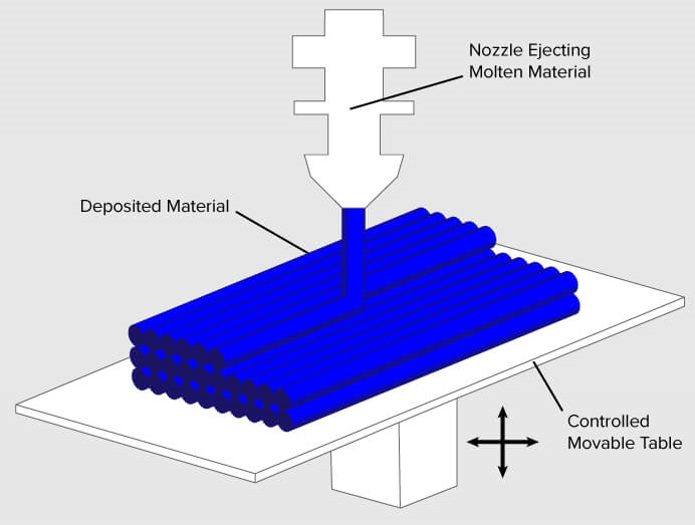
\includegraphics[width=10cm]{kapitel3/fdm}
  \caption{Visualisierung des FDM-Verfahrens}
  \source{\url{https://3dprinting.com/what-is-3d-printing/}}
  \label{Kap3:FDM}
\end{figure}

\subsection{Einstellmöglichkeiten}

\TODO

\section{Infill}

\subsection{Infill-Muster}